\section{例子展示}

% 插入图片
……显示图片
\begin{figure}[H]
    \begin{center}
        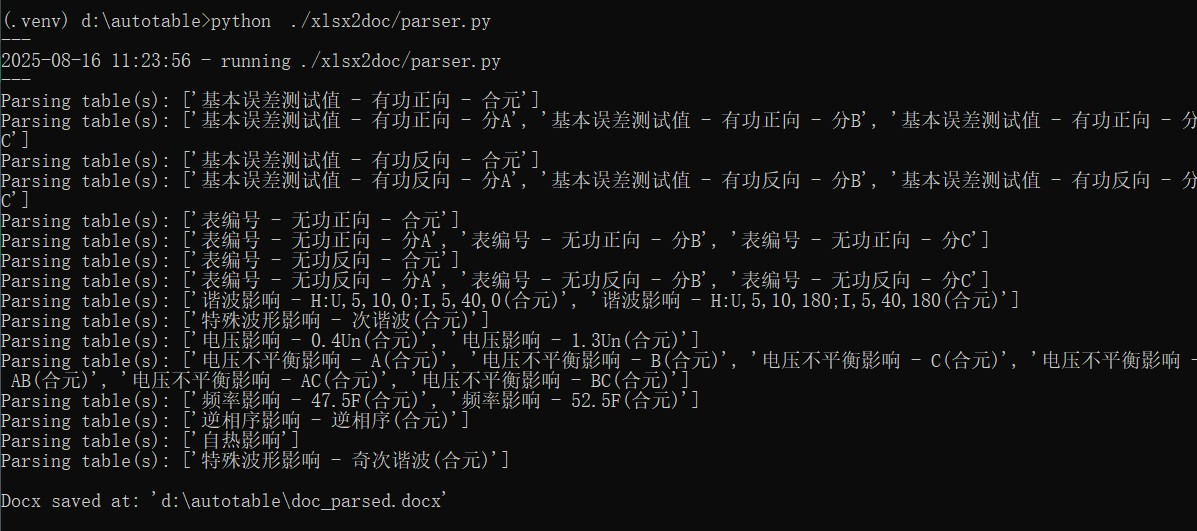
\includegraphics[width=.95\linewidth]{res/results.jpg}\\
        \caption{TOU aglomerado 3 dias Barracão de 5 a 12 de dezembro de 2024.}\label{01}
    \end{center}
\end{figure}

% 插入item
……插入item

%\vspace{-.7cm}
\begin{enumerate}
    \item selecione no menu de ferramentas a opção citada;
    \item clique sobre a camada "paranaUTM";
    \item selecione dois pontos no mapa para fazer a medição.
\end{enumerate}

% 插入item2
……插入item2

%\vspace{-.7cm}
    \begin{itemize}
        \item how to access Qgisweb from the Zabbix tool;
        \item introdução ao uso do QGIS; navegação pelo mapa; 
        \item instruções detalhadas sobre a ferramenta Hxmap; 
    \end{itemize}

% 插入公式
……插入公式

\[S_n = \frac{X_1 + X_2 + \cdots + X_n}{n}
      = \frac{1}{n}\sum_{i}^{n} X_i\]

% 插入代码
……插入代码

\begin{minted}[frame=lines,framesep=1mm]{python}
% 插入类似python和html等高亮代码
# 读取文件
import os, json

def load_user(file_path):
    with open(file_path, "r", encoding="utf-8") as f:
        return json.load(f)

users = load_user("users.json")
print(f"{len(users)}名用户已成功加载。")
\end{minted}

% 插入bash等的命令行代码高亮
\begin{lstlisting}
# 在项目目录里运行命令
(.venv) d:\autotable>python  ./xlsx2doc/parser.py
\end{lstlisting}


% 插入表格
…… 插入表格
\begin{table}[ht]
    \centering
    \caption{实验结果对比}
    \begin{tabular}{lccc}
        \toprule
        方法 & 指标1 & 指标2 & 指标3 \\
        \midrule
        方法A & 0.123 & 0.234 & 0.345 \\
        方法B & 0.456 & 0.567 & 0.678 \\
        \bottomrule
    \end{tabular}
    \label{tab:results}
\end{table}

% 插入大括号
...通讯状态
\[ 
comStatus= \left\{
\begin{array}{ll}
    veryGood: comAvg \geq 98\%\\
    good: 98\% > comAvg \geq 75\%\\
    ok: 75\% > comAvg \geq 50\%\\
    bad: 50\% > comAvg \geq 25\%\\
    veryBad: 25\% > comAvg > 0\%\\
    zero: comAvg = 0\%\\
\end{array} 
\right. 
\]
